%%% Template by Mikhail Klassen, April 2013
%%% 
\documentclass[11pt,letterpaper]{article}
\newcommand{\workingDate}{\textsc{2019 $|$ April $|$ 2}}
\newcommand{\userName}{Jordan Sturtz}
\newcommand{\institution}{ Oregon State University} \usepackage{researchdiary_png}
\usepackage{listings, lstautogobble}
\usepackage{graphicx}
\usepackage{wrapfig}
\usepackage{enumitem}

\lstset{
  autogobble=true, 
  breaklines=true
}

% To add your univeristy logo to the upper right, simply
% upload a file named "logo.png" using the files menu above.

\begin{document} \univlogo

\title{CS 362 - Assignment 3}
{\Huge Assignment 3}\\[5mm]
\begin{enumerate}[label=\Roman*.]
  \item \textbf{Unit Testing}
    
    For all my unit tests, I first came up with some input partitioning scheme
    to better increase my test coverage. For example, cards that draw from the
    deck might behave differently in code if they draw into an empty deck that
    must be shuffled from discard. So, my tests must cover multiple input cases. 
    Each of the subsections below will detail the specific input cases I tested. 
    I could not test all the cases that I conceived, 
    but I hope my selections are meet the project requirements. 

    For every unit test, some tests are not 
    input dependent, i.e. they test variables that should change regardless of
    input type. For example, regardless of whether the Council Room draws from
    an empty deck, it must increase the number of buys for the player by 1. 
    Therefore, the subsections below will detail the Input Independent tests
    and the Input Dependent tests. 

    For the cards that I tested both by calling cardEffect and by calling
    the refactored code directly (e.g. adventurer and smithy), I tested
    different input. Because there are input independent tests, there is
    some repeat code since these are input independent tests. Rather than
    repeat the documentation for these repeat tests, I will note when they
    are identical with "Same as Above."

    \begin{itemize}[leftmargin=*]
      \item \textbf{Unittest1 - AdventurerEffect}
        
        \begin{itemize}[leftmargin=*, label={}]
          \item \textbf{Input Independent Tests}

            \begin{itemize}[leftmargin=*]
              \item Adventurer card should be "played" i.e. added to playedCard variable
              \item Player's hand should be increased by 1 (draw two treasures, play adventurer)
              \item The two new cards should be treasures
              \item Player's original hand has not been changed (aside from two new treasures and playing Adventurer)
              \item Player's card count has not changed (i.e. deck + discard + hand + played stays the same)
              \item Gamestate has not changed for any non-player related variables
              \item Gamestate has not changed for any other player
            \end{itemize}

          \item \textbf{Input Dependent Tests}
          \item If the first two cards of the deck are treasures: 
            \begin{itemize}[leftmargin=*]
              \item Discard pile has not changed
              \item Deckcount decreased by two
            \end{itemize}
          \item If the first two cards are not treasures but there are two treasures in deck (i.e. no shuffle required to reveal treasures)
            \begin{itemize}[leftmargin=*]
              \item Discard pile has not changed
              \item Deckcount decreased by amount equal to second location of treasure in deck
            \end{itemize}
        \end{itemize}

      \item \textbf{Cardtest1 - cardEffect with adventurer}
        \begin{itemize}[leftmargin=*, label={}]
          \item \textbf{Input Independent Tests (Same as above)}
          \item \textbf{Input Dependent Tests}
          \item If there is are less than two treasures in deck:
            \begin{itemize}[leftmargin=*]
              \item Discard pile should not have any treasures (otherwise, a treasures was discarded)
            \end{itemize}
        \end{itemize}

      \item \textbf{Unittest2 - SmithyEffect}

        \begin{itemize}[leftmargin=*, label={}]
          \item \textbf{Input Independent Tests}

            \begin{itemize}[leftmargin=*]
              \item Player's hand should be increased by 2 (draw three, subtract 1 for playing smithy)
              \item Player's original hand should not have changed(aside from new cards and playing smithy)
              \item Player's total card count has not changed (i.e. deck + discard + hand + played stays the same)
              \item Gamestate has not changed for any non-player variable
              \item Gamestate has not changed for any other player
            \end{itemize}

          \item \textbf{Input Dependent Tests}
          \item If the deck has more than three cards: 
            \begin{itemize}[leftmargin=*]
              \item New cards in hand should be same as top three cards in deck
              \item DeckCount should decrease by three
              \item Discard pile should not change
            \end{itemize}
        \end{itemize}

      \item \textbf{Cardtest2 - cardEffect with Smithy}
        \begin{itemize}[leftmargin=*, label={}]
          \item \textbf{Input Independent Tests (Same as above)}
          \item \textbf{Input Dependent Tests}
          \item If deck has less than three cards left: 
            \begin{itemize}[leftmargin=*]
              \item Hand should have all cards currently in deck
              \item Discard pile should be empty because of reshuffle
            \end{itemize}
        \end{itemize}

      \item \textbf{Unittest3 - CouncilRoomEffect}

        \begin{itemize}[leftmargin=*, label={}]
          \item \textbf{Input Independent Tests}

            \begin{itemize}[leftmargin=*]
              \item Player's hand should be increased by 3 (draw four, play council room)
              \item Player's original hand has not been changed (aside from card draws and playing council room)
              \item Player's card count has not changed (i.e. deck + discard + hand + played stays the same)
              \item Gamestate has not changed except +1 Buy
              \item Other players' hand increased by 1
              \item New card in each non-active player's hand should come from top of their decks
            \end{itemize}

          \item \textbf{Input Dependent Tests}
          \item If both the active player (the one playing the card) and the inactive player have enough cards in deck to draw +3 and +1 respectively:
            \begin{itemize}[leftmargin=*]
              \item For active player, new cards in hand should be same as top three cards in deck
              \item For active player, deckCount should decrease by three
              \item For active player, discard pile should not change
              \item For inactive player, new card in hand should be same as top of player's deck
              \item For inactive player, deckCount should decrease by 1
              \item For inactive player, discard pile should not change
            \end{itemize}
          \item If the active player has fewer than four cards in deck and inactive player has exactly 0 (i.e. both must shuffle):
            \begin{itemize}[leftmargin=*]
              \item For active player, any cards left in deck should be in hand
              \item For active player, discard pile should be empty
              \item For inactive player, discard pile should be empty
            \end{itemize}
        \end{itemize}

      \item \textbf{Cardtest3 - cardEffect with Great Hall}
        \begin{itemize}[leftmargin=*, label={}]
          \item \textbf{Input Independent Tests}
            \begin{itemize}[leftmargin=*]
              \item Player's handCount should not change (+1 Card negated by playing Great Hall)
              \item Player's original hand has not been changed (aside from +1 Card and playing Great Hall)
              \item Player's total card count has not changed (i.e. deck + discard + hand + played stays the same)
              \item Gamestate has not changed except +1 Actions
              \item Other player variables have not changed
              \item Great Hall card should be played, i.e. added to playedCards array
            \end{itemize}
          \item \textbf{Input Dependent Tests}
          \item If deck has greater than zero cards left: 
            \begin{itemize}[leftmargin=*]
              \item Hand should have same card as top of deck
              \item DeckCount should decrease by 1
              \item Discard pile should not change
            \end{itemize}
          \item If deck has exactly zero cards left:
            \begin{itemize}[leftmargin=*]
              \item Discard pile should be empty
            \end{itemize}
        \end{itemize}

      \item \textbf{Unittest4 - villageEffect}

        \begin{itemize}[leftmargin=*, label={}]
          \item \textbf{Input Independent Tests}

            \begin{itemize}[leftmargin=*]
              \item Village card should be played, i.e. added to playedCards array
              \item Player's hand should not change (+1 Card negated by playing Village)
              \item Player's original hand has not been changed (except for +1 Card and playing Village)
              \item Player's total card count has not changed (i.e. deck + discard + hand + played stays the same)
              \item Gamestate has not changed except +2 Actions
              \item Other player variables have not changed
            \end{itemize}

          \item \textbf{Input Dependent Tests}
          \item If the deck has more than zero cards left: 
            \begin{itemize}[leftmargin=*]
              \item Hand should have same card as top of deck
              \item DeckCount should decrease by 1
              \item Discard pile should not change
            \end{itemize}
          \item If the deck has exactly zero cards:
            \begin{itemize}[leftmargin=*]
              \item Discard pile should be empty
            \end{itemize}
        \end{itemize}

      \item \textbf{Cardtest4 - cardEffect with Mine}
        \begin{itemize}[leftmargin=*, label={}]
          \item \textbf{Input Independent Tests (None)}
          \item \textbf{Input Dependent Tests}
          \item If the handposition of the card selected for trashing is a treasure and the card selected for gaining is also a treasure: 
            \begin{itemize}[leftmargin=*]
              \item Player's handCount decrease by 1 (by playing Mine)
              \item Chosen card should be replaced with treasure no more than +3 its cost
              \item Player's total card count has not changed (i.e. deck + discard + hand + played stays the same)
              \item Supply pile from gained treasure should decrease by 1
              \item Gamestate variables unrelated to player should not change 
              \item Other player variables should not change
              \item Mine card should be played, i.e. added to playedCards array
              \item Discard pile should not change
            \end{itemize}
          \item If a non-treasure is selected for trashing:
            \begin{itemize}[leftmargin=*]
              \item Function should return -1
              \item Gamestate should be unaltered
            \end{itemize}
          \item If a non-treasure is selected for gaining:
            \begin{itemize}[leftmargin=*]
              \item Function should return -1
              \item Gamestate should be unaltered
            \end{itemize}
        \end{itemize}
    \end{itemize}

  \item \textbf{Bugs}

    \begin{enumerate}
      \item \textbf{unitest1.c/cardtest1.c - Adventurer}
        
        \begin{itemize}[leftmargin=*]

        \item \textbf{Play Card Bug}:

        \textbf{Description of Bug}: When the adventurer card is played, it does
          not appear at the top of the playedCard array.

        \textbf{How to Cause}: Initialize a game, add an adventurer card to 
          the first player's hand, and then call adventureEffect with the correct
          hand position. Then check that (a) playedCardCount has increased by
          1 and that (b) the top of playedArray is adventurer.

        \textbf{Code}:
          \begin{lstlisting}
int main() {
  // INITIALIZATION HERE
  int pass;                             
  int seed = 1000;                      
  int numPlayers = 4;                   
  int player = 0;                       
  int handpos;                          
  struct gameState G, testG, blankG;    

  // initialize a game state and player cards
  int k[10] = {adventurer, embargo, village, minion, mine, cutpurse, sea_hag, tribute, smithy, council_room}; initializeGame(numPlayers, k, seed, &G);
  memcpy(&blankG, &G, sizeof(struct gameState));

  G.deck[player][G.deckCount[player]] = gold;         
  G.deck[player][G.deckCount[player]+1] = province;
  G.deck[player][G.deckCount[player]+2] = silver;
  G.deck[player][G.deckCount[player]+3] = duchy;
  G.deckCount[player] = G.deckCount[player] + 4;

  handpos = G.handCount[player];                     
  G.hand[player][handpos] = adventurer;     
  G.handCount[player]++;                                
  
  memcpy(&testG, &G, sizeof(struct gameState));         
  adventurerEffect(&testG, player, handpos);                     
  
  // TEST STARTS HERE
  if (testG.playedCardCount == G.playedCardCount + 1) {
    if (testG.playedCards[testG.playedCardCount - 1] == adventurer)
      printf("\tPASSED: Adventurer card was properly played, i.e. smithy added to playedCard array\n");
    else
      printf("\t\u274CFAILED: Adventurer card was not properly played, i.e. added to playedCard array\n");
  } 
  else printf("\t\u274CFAILED: Adventurer card was not properly played, i.e. added to playedCard array\n");
}
          \end{lstlisting}

        \item \textbf{Hand Count Bug}

        \textbf{Description of Bug}: Handcount increases by 2 instead of 1

        \textbf{How to Cause}: Initialize a game, add an adventurer card to 
          the first player's hand, and then call adventureEffect with the correct
          hand position. Then check that handcount has increased by two.

        \textbf{Code}:
          \begin{lstlisting}
int main() {

  ...<initialization same as above>...
    int oldCount = G.handCount[player];
    int newCount = testG.handCount[player];
    if (oldCount + 1 == newCount) printf("\tPASSED: HandCount increased by 1 (2 treasures - 1 adventurer)\n"); 
    else printf("\t\u274CFAILED: Handcount should have increased by 1, instead increased by %d\n", newCount - oldCount);

}
          \end{lstlisting}

        \item \textbf{Total Card Count Bug}:

          \textbf{Description of Bug}: The total card count of the player (deck + discard + hand + played)
            does not stay the same after calling the function. This bug does not appear when the top
            two cards are treasures, but does appear when there are any non-treasures between the top
            of the deck and the second treasure in the deck.

        \textbf{How to Cause}: Initialize a game, add an adventurer card to the first player's hand, 
            add some non-treasures to deck, and then run the function and compare. 

        \textbf{Code}:
          \begin{lstlisting}
int main() {

  ...<initialization same as above>...
  int gCount = G.deckCount[player] + G.discardCount[player] + G.handCount[player] + G.playedCardCount;
  int testGCount = testG.deckCount[player] + testG.discardCount[player] + testG.handCount[player] + testG.playedCardCount;
  
  if (gCount == testGCount)
    printf("\tPASSED: Total card count is the same: deck + discard + hand + played\n");
  else if (gCount < testGCount)
    printf("\t\u274CFAILED: Total card count of deck (deck + discard + hand + played) less than after card effect\n"); 
  else
    printf("\t\u274CFAILED: Total card count of deck (deck + discard + hand + played) greater than after card effect\n");
}
          \end{lstlisting}

        \item \textbf{Discard Count Bug}:

          \textbf{Description of Bug}: The discard count increase does not match the number of 
          non-treasures drawn from deck. This bug is only detectable when (1) there are non-treasures
          in the deck before the second treasure and (2) there are at least two treasures in 
          the deck. 

        \textbf{How to Cause}: Initialize a game, add an adventurer card to the first player's hand, 
            add two treasures to the deck followed by two non-treasures. Check to see if discard pile has increased by 2.

        \textbf{Code}:
          \begin{lstlisting}

 ...<initialization same as above>... 
  if (testG.discardCount[player] == G.discardCount[player] + 2) {
    int first = testG.discard[player][testG.discardCount[player] - 1];
    int second = testG.discard[player][testG.discardCount[player] - 2];

    if ((first == duchy) && (second == province))
      printf("\tPASSED: Discarded cards match non-treasures drawn from deck\n");
    else
      printf("\t\u274CFAILED: Discarded cards do not match non-treasures drawn from deck\n");
  }
  else printf("\t\u274CFAILED: Discard should have increased by 2, but instead increased by %d\n", testG.discardCount[player] - G.discardCount[player]);
}
\end{lstlisting}

        \end{itemize}

      \item \textbf{unitest2.c/cardtest2.c - Smithy}

        \begin{itemize}[leftmargin=*]

        \item \textbf{Number Buys Bug}:

        \textbf{Description of Bug}: When the Smithy card is played, it increases
            the number of buys for the player.

        \textbf{How to Cause}: Initialize a game, add an Smithy card to 
          the first player's hand, and then call smithyEffect with the correct
          hand position. Test the state of the game to see if numBuys has increased.

        \textbf{Code}:

          \begin{lstlisting}

int main() {
  
  int pass;                             
  int seed = 1000;                      
  int numPlayers = 4;                   
  int player = 0;                      
  struct gameState G, testG;  
  int handpos = 4;                   

  // initialize a game state and player cards
  int k[10] = {adventurer, embargo, village, minion, mine, cutpurse, sea_hag, tribute, smithy, council_room};
  initializeGame(numPlayers, k, seed, &G);
  memcpy(&testG, &G, sizeof(struct gameState));
  smithyEffect(&testG, player, handpos);       

  if (G->numBuys != testG->numBuys) {
    printf("\t\u274CFAILED: Gamestate numBuys has changed\n");
    total_pass = 0;
  }
}
          \end{lstlisting}
        \end{itemize}

      \item \textbf{unitest3.c - Council Room}

        \begin{itemize}[leftmargin=*]

        \item \textbf{Handcount Bug}:

        \textbf{Description of Bug}: Handcount should always increase by three 
            for a player that plays council room. This is because the player should 
            draw four cards and then "play" council room which reduces handcount by 1.
            The handcount is off for the active player but is correct for the other players
            who must draw 1.

        \textbf{How to Cause}: Initialize a game, add an council room card to 
          the first player's hand, and then call councilRoomEffect with the correct
          hand position. Test the state of the game to see how much hand count has increased.

        \textbf{Code}:

          \begin{lstlisting}
int main() {
  
  int seed = 1000;                      
  int numPlayers = 2;                   
  int player = 0;                       
  struct gameState G, testG;
  int handpos = 4;                      

  int k[10] = {adventurer, embargo, village, minion, mine, cutpurse, sea_hag, tribute, smithy, council_room};
  initializeGame(numPlayers, k, seed, &G);

  memcpy(&testG, &G, sizeof(struct gameState)); 
  councilRoomEffect(&testG, player, handpos);   

  int oldCount = G.handCount[player];
  int newCount = testG.handCount[player];
  if (oldCount + X == newCount) printf("\tPASSED: For Player %d, HandCount increased by %d\n", player, X); 
  else printf("\t\u274CFAILED: For Player %d, expected handcount to increase by %d, but increased by %d\n", player, X, newCount - oldCount);

          \end{lstlisting}

        \item \textbf{Hand Matches Deck}:

        \textbf{Description of Bug}: The top four cards in a deck should match the
            top four cards in the player's hand. In fact, the top four cards do not
            match because the code only draws three cards.

        \textbf{How to Cause}: Initialize a game, add an council room card to 
          the first player's hand, and then call councilRoomEffect with the correct
          hand position. Test the state of the game to see if top four cards of hand
            match top four cards of deck.

        \textbf{Code}:

          \begin{lstlisting}
int main() {
  
  ... <initialization code same as above> ...
  int pass = 1;
  for (int i = 0; i < 4; i++) {
    int handCard = testG.hand[player][G.handCount[player] - 1 + i];
    int deckCard = G.deck[player][G.deckCount[player] - 1 - i];
    if (handCard != deckCard) {
      pass = 0;
    }
  }
  if (pass) printf("\tPASSED: Cards added to hand match top four cards of deck\n");
  else printf("\t\u274CFAILED: Cards added to hand do not match top four cards of deck\n");

          \end{lstlisting}

        \item \textbf{Deck Does not Decrease by Four}:

        \textbf{Description of Bug}: The player's deck should decrease by four in the case
        where there is are at least four cards in the deck. In fact, the deck only decreases
        by three.

        \textbf{How to Cause}: Initialize a game, add an council room card to 
          the first player's hand, and then call councilRoomEffect with the correct
          hand position. Test the state of the game to see if deck decreases by four.

        \textbf{Code}:

          \begin{lstlisting}
int main() {
  
  ... <initialization code same as above> ...

  if (G.deckCount[player] == testG.deckCount[player] + 4) 
    printf("\tPASSED: For player 0, deck has decreased by exactly four\n");
  else
    printf("\t\u274CFAILED: For player 0, deck has not decreased by exactly four\n");
}
          \end{lstlisting}

        \item \textbf{Discard is not Empty }:

        \textbf{Description of Bug}: The discard is not empty after calling council room
        with fewer than four cards.

        \textbf{How to Cause}: Initialize a game, add an council room card to 
          the first player's hand, set the deck so that it has only three cards, 
          and then call councilRoomEffect with the correct
          hand position. Test the state of the game to see if discard is empty, 
          which would imply that the deck was shuffled.

        \textbf{Code}:

          \begin{lstlisting}
int main() {
  
  ... <initialization code same as above> ...

  setDeck(&G, player, 3); // will set deck with only three coppers, and discard with ten coppers
  memcpy(&testG, &G, sizeof(struct gameState));         
  councilRoomEffect(&testG, player, handpos); 

  if (testG.discardCount[player] == 0)
    printf("\tPASSED: discard count is 0\n");
  else
    printf("\t\u274CFAILED: discard count is not 0\n");
}
          \end{lstlisting}


        \end{itemize}

      \item \textbf{unitest4.c - Village (No Bugs)}
      \item \textbf{cardtest3.c - Great Hall}

        \begin{itemize}[leftmargin=*]

        \item \textbf{Total Card Count Bug}:

        \textbf{Description of Bug}: Total card count of deck is less after
            this card is used. Bug shows up regardless of whether deck must
            be shuffled.

        \textbf{How to Cause}: Initialize a game, add an great hall card to 
          the first player's hand, and then call cardEffect.
          Test the state of the game to see if total card count has changed.

        \textbf{Code}:

          \begin{lstlisting}
int main() {
  
  int seed = 1000;                      
  int numPlayers = 2;                   
  struct gameState G, testG;   
  int handpos = 4;                    
  int player = 0;                    
  int coin_bonus = 0;

  int k[10] = {adventurer, embargo, village, minion, mine, cutpurse, sea_hag, tribute, smithy, council_room};
  initializeGame(numPlayers, k, seed, &G);
  memcpy(&testG, &G, sizeof(struct gameState)); 
  cardEffect(great_hall, 0, 0, 0, &testG, handpos, &coin_bonus); 

  int gCount = G.deckCount[player] + G.discardCount[player] + G.handCount[player] + G.playedCardCount;
  int testGCount = testG.deckCount[player] + testG.discardCount[player] + testG.handCount[player] + testG.playedCardCount;
  
  if (gCount == testGCount)
    printf("\tPASSED: Total card count is the same\n");
  else if (gCount < testGCount)
    printf("\t\u274CFAILED: Total card count of deck less than after card effect\n"); 
  else
    printf("\t\u274CFAILED: Total card count of deck greater than after card effect\n");
 
          \end{lstlisting}

        \item \textbf{Played Card Bug}:

        \textbf{Description of Bug}: Does not add itself to playedCard array.
            Bug shows up regardless of whether deck is shuffled from discard.

        \textbf{How to Cause}: Initialize a game, add an great hall card to 
          the first player's hand, and then call cardEffect.
          Test the state of the game to see if card was added to playedCards.

        \textbf{Code}:

          \begin{lstlisting}
int main() {
  
  ... <same initialization code as above> ...

  if (testG.playedCardCount == G.playedCardCount + 1) {
    if (testG.playedCards[testG.playedCardCount - 1] == great_hall)
      printf("\tPASSED: Great Hall card was properly played, i.e. added to playedCard array\n");
    else
      printf("\t\u274CFAILED: Great Hall card was not properly played, i.e. added to playedCard array\n");
  } 
  else printf("\t\u274CFAILED: Great Hall card was not properly played, i.e. added to playedCard array\n");
          \end{lstlisting}
        \end{itemize}

      \item \textbf{cardtest4.c - Mine}

        \begin{itemize}[leftmargin=*]

        \item \textbf{Total Card Count Bug}:

        \textbf{Description of Bug}: Total card count of deck is greater than after
            this card is used. Bug shows up regardless of whether deck must
            be shuffled.

        \textbf{How to Cause}: Initialize a game, add an Mine card to 
          the first player's hand, and then call cardEffect.
          Test the state of the game to see if total card count has changed.

        \textbf{Code}:

          \begin{lstlisting}
int main() {
  
  int seed = 1000;                      
  int numPlayers = 2;                   
  struct gameState G, testG;   
  int handpos = 4;                    
  int player = 0;                    
  int coin_bonus = 0;
  int choice0, choice1;  
  int result;            

  int k[10] = {adventurer, embargo, village, minion, mine, cutpurse, sea_hag, tribute, smithy, council_room};
  initializeGame(numPlayers, k, seed, &G);
  setHand(&G, player, handpos); // sets hand to have four coppers and Mine
  choice0 = 0;                  // will be trashing first copper
  choice1 = silver;             // will be gaining silver 
  memcpy(&testG, &G, sizeof(struct gameState)); 
  cardEffect(mine, choice0, choice1, 0, &testG, handpos, &coin_bonus); 
  
  // TEST STARTS HERE
  int gCount = G.deckCount[player] + G.discardCount[player] + G.handCount[player] + G.playedCardCount;
  int testGCount = testG.deckCount[player] + testG.discardCount[player] + testG.handCount[player] + testG.playedCardCount;
  
  if (gCount == testGCount)
    printf("\tPASSED: Total card count is the same\n");
  else if (gCount < testGCount)
    printf("\t\u274CFAILED: Total card count of deck less than after card effect\n"); 
  else
    printf("\t\u274CFAILED: Total card count of deck greater than after card effect\n");
          \end{lstlisting}

        \item \textbf{Played Card Bug}:

        \textbf{Description of Bug}: Does not add itself to playedCard array.

        \textbf{How to Cause}: Initialize a game, add a Mine hall card to 
          the first player's hand, and then call cardEffect.
          Test the state of the game to see if card was added to playedCards.

        \textbf{Code}:

          \begin{lstlisting}
int main() {
  
  ... <same initialization code as above> ...

  if (testG.playedCardCount == G.playedCardCount + 1) {
    if (testG.playedCards[testG.playedCardCount - 1] == mine)
      printf("\tPASSED: Mine was properly played, i.e. added to playedCard array\n");
    else
      printf("\t\u274CFAILED: Mine was not properly played, i.e. added to playedCard array\n");
  } 
  else printf("\t\u274CFAILED: Mine was not properly played, i.e. added to playedCard array\n");
          \end{lstlisting}

        \item \textbf{Attempting to Gain Treasure Does not Return -1}:

        \textbf{Description of Bug}: The code does not return -1 when the
        cardEffect function is called with a non-treasure as the card to be
        gained. As a result, this bug alters the gameState by continuing
        to execute the mine cardEffect.

        \textbf{How to Cause}: Initialize a game, add an Mine card to 
          the first player's hand, and then call cardEffect.
          Call this function with choice1 set to a non-treasure.

        \textbf{Code}:

          \begin{lstlisting}
int main() {
  
  int seed = 1000;                      
  int numPlayers = 2;                   
  struct gameState G, testG;   
  int handpos = 4;                    
  int player = 0;                    
  int coin_bonus = 0;
  int choice0, choice1;  
  int result;            

  int k[10] = {adventurer, embargo, village, minion, mine, cutpurse, sea_hag, tribute, smithy, council_room};
  initializeGame(numPlayers, k, seed, &G);
  setHand(&G, player, handpos); // sets hand to have four coppers and Mine
  choice0 = 0;                  // will be trashing first copper
  choice1 = village;             // NOT ALLOWED
  memcpy(&testG, &G, sizeof(struct gameState)); 
  
  // TEST STARTS HERE
  result = cardEffect(mine, choice0, choice1, 0, &testG, handpos, &coin_bonus);
  if (result == -1)
    printf("\tPASSED: Function returned -1 (not allowed to trash non-treasure)\n");
  else printf("\t\u274CFAILED: Function did not return -1, so it continued unexpectedly\n");
          \end{lstlisting}
        \end{itemize}
    \end{enumerate}

  \item \textbf{Code Coverage}
    
    \begin{itemize}[leftmargin=*]
      \item \textbf{Unittest1 - AdventureEffect}
      
        \begin{enumerate}[leftmargin=*]
          \item \textbf{Statement and Branch Coverage}

          \begin{lstlisting}
          Function 'adventurerEffect'
          Lines executed:94.12% of 17
          Branches executed:100.00% of 12
          Taken at least once:83.33% of 12
          Calls executed:50.00% of 2
          \end{lstlisting}

          The percent lines executed is not 100\% because the code in unittest1.c
          does not test the following code snippet within adventureEffect:

          \begin{lstlisting}
        if (state->deckCount[currentPlayer] <1){
          shuffle(currentPlayer, state);
        }
          \end{lstlisting}

          That statement is executed in the tests run in cardtest1.c. This is because of how
            I divided the input cases. Unittest1.c tests cases where no shuffle is needed, 
            and cardtest1.c tests cases where a shuffle is required. 
            \begin{figure}
            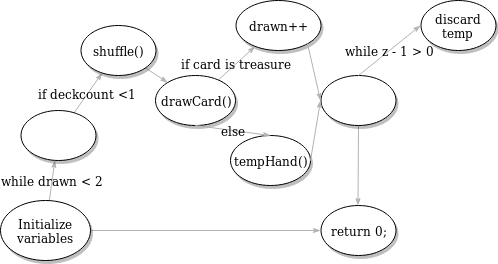
\includegraphics[width=\textwidth]{unittest1}
              \caption{Node coverage figure for adventureEffect}
            \end{figure}

        \item \textbf{Input Coverage and Boundary Cases}

          I did not have time to test many other input cases. Some of these cases are tricky because
            they require inferring what the behavior of the system should be from the source code itself. 
            Given more time, I would test the following: 
          \begin{itemize}
            \item Inputs where function is given invalid values for player or handpos. What
                should the function do in these cases? It is not clear from a development
                standpoint, and therefore unclear from a testing standpoint. 
            \item A case where there are multiple adventurer cards in hand. Does this create
              undesirable behavior?
            \item A case where there is only one adventurer card in hand.
            \item A case where there are no treasures in deck or discard (could happen if a player trashes enough treasures)
            \item A case where the function is called when the hand is at MAX\_HAND number of cards (and therefore, hand would exceed MAX\_HAND)
          \end{itemize}
        \end{enumerate}

      \item \textbf{Cardtest1 - cardEffect on Adventure}
      
        \begin{enumerate}[leftmargin=*]
          \item \textbf{Statement and Branch Coverage}
          \begin{lstlisting}
          Function 'adventurerEffect'
          Lines executed:100.00% of 17
          Branches executed:100.00% of 12
          Taken at least once:83.33% of 12
          Calls executed:100.00% of 2
          \end{lstlisting}

          Unlike unittest1.c, since these tests cause the adventurerEffect function
            to shuffle, it acheives 100\% code coverage.

        \item \textbf{Input Coverage and Boundary Cases}
          
          In addition to the above tests, since this code is testing the cardEffect 
            function itself which calls adventurerEffect, I would also add the following
            tests:
          \begin{itemize}
            \item The function should not behave any differently if coin\_bonus is 
              a different value. 
            \item The function should do nothing special if choice0, choice1, or choice3 
              are values other than 0, since adventurer does not have a optional effect.
          \end{itemize}
        \end{enumerate}

      \item \textbf{Unittest2 - smithyEffect}
        \begin{enumerate}[leftmargin=*]
          \item \textbf{Statement and Branch Coverage}

          \begin{lstlisting}
          Function 'smithyEffect'
          Lines executed:100.00% of 6
          Branches executed:100.00% of 2
          Taken at least once:100.00% of 2
          Calls executed:100.00% of 2
          \end{lstlisting}

          The percent lines executed 100\% because the smithyEffect function
          has no conditional branches. As such, no conditional branching node
          diagram is needed. Every call to smithyEffect is guaranteed to 
          execute all branches and all statements. However, it should be
          noted that smithyEffect calls drawCard, which has much worse
          coverage: 

          \begin{lstlisting}
          Function 'drawCard'
          Lines executed:36.36% of 22
          Branches executed:33.33% of 6
          Taken at least once:16.67% of 6
          Calls executed:0.00% of 1
          \end{lstlisting}

        \item \textbf{Input Coverage and Boundary Cases}
          
          For unittest2.c, I only tested one input: a case where the deck has more
            than three cards in it. In cardtest2.c, I tested a case where the deck must be
            reshuffled from discard to access the next cards in deck. Since this logic
            is handled in drawCard, failures unique to this case are likely related to 
            failures in drawCard. Given more time, I would test the following cases in a
            more throughout unit test:
          \begin{itemize}
            \item Inputs where function is given invalid values for player or handpos. What
                should the function do in these cases? It is not clear from a development
                standpoint, and therefore unclear from a testing standpoint. 
            \item A case where there are multiple smithy cards in hand. Does this create
              undesirable behavior?
            \item A case where there is only one smithy card in hand.
            \item A case where the function is called when the hand is at MAX\_HAND number of cards (and therefore, hand would exceed MAX\_HAND)
          \end{itemize}
        \end{enumerate}

      \item \textbf{Cardtest2 - cardEffect with Smithy}
        \begin{enumerate}[leftmargin=*]
          \item \textbf{Statement and Branch Coverage}
          
          As mentioned above, the statement and branch execution will be
          100\% since there are no conditional branches in smithyEffect.

        \item \textbf{Input Coverage and Boundary Cases}
          
          Since this test calls smithyEffect from cardEffect, I would add the above tests
            to test this function:
          \begin{itemize}
            \item The function should not behave any differently if coin\_bonus is 
              a different value. 
            \item The function should do nothing special if choice0, choice1, or choice3 
              are values other than 0, since smithy does not have a optional effect.
          \end{itemize}
        \end{enumerate}

      \item \textbf{Unittest3 - Council Room}
      
        \begin{enumerate}[leftmargin=*]
          \item \textbf{Statement and Branch Coverage}

          \begin{lstlisting}
          Function 'councilRoomEffect'
          Lines executed:100.00% of 9
          Branches executed:100.00% of 6
          Taken at least once:100.00% of 6
          Calls executed:100.00% of 3
          \end{lstlisting}
          
            The percent lines and branches executed are 100\% because the way that the
            code is designed in councilRoomEffect guarantees that all branches
            and all statements are covered for every execution. There is only
            one conditional branch inside a for-loop below that is guaranteed
            to execute once during the loop which means that all branches
            and statements will be covered:

          \begin{lstlisting}
          for (i = 0; i < state->numPlayers; i++) {
            if ( i != currentPlayer )
              drawCard(i, state);
          }
          \end{lstlisting}

            \begin{figure}
            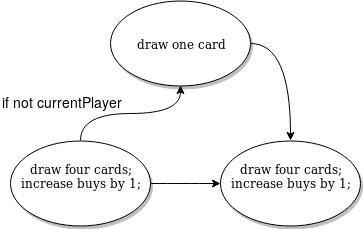
\includegraphics[width=\textwidth]{unittest3}
              \caption{Node graph figure for councilRoomEffect}
            \end{figure}

        \item \textbf{Input Coverage and Boundary Cases}

          I covered two major cases involving the deck: the first is when the deck size is greater than
            four and the second is when the decksize is less than four. A boundary case worth considering
            is the case when the decksize is precisely four. In this case, it is important for testers
            to consider whether the intended behavior of the system is to shuffle the deck immediately
            when the deck is emptied or if instead the system should shuffle the deck only when prompted
            to draw from the empty pile. Some other inputs I would check in a more thorough system are:
          \begin{itemize}
            \item Inputs where function is given invalid values for player or handpos. What
                should the function do in these cases? It is not clear from a development
                standpoint, and therefore unclear from a testing standpoint. 
            \item A case where there are multiple council room cards in hand. Does this create
              undesirable behavior?
            \item A case where there is only one council room card in hand.
            \item A case where the function is called when the hand is at MAX\_HAND number of cards (and therefore, hand would exceed MAX\_HAND)
          \end{itemize}
        \end{enumerate}

      \item \textbf{Unittest4 - Village}
      
        \begin{enumerate}[leftmargin=*]
          \item \textbf{Statement and Branch Coverage}

          \begin{lstlisting}
          Function 'villageEffect'
          Lines executed:100.00% of 5
          No branches
          Calls executed:100.00% of 2
          \end{lstlisting}
          
            There are only three statements in villageEffect, two of which are
            function calls. Therefore, the coverage is 100\%.

        \item \textbf{Input Coverage and Boundary Cases}

          I covered two major cases involving the deck: the first is when the deck size is empty and 
            the second is when the deck has exactly one card. My assumption based on analyzing the
            code is that it is acceptable for the deck to be empty. Only when a function requires
            drawing from an empty deck does it prompt the system to reshuffle the deck from discard.
            For both input cases, the tests all came back as passed. More thorough testing might
            include the following tests:
          \begin{itemize}
            \item Inputs where function is given invalid values for player or handpos. What
                should the function do in these cases? It is not clear from a development
                standpoint, and therefore unclear from a testing standpoint. 
            \item A case where there are multiple village cards in hand. Does this create
              undesirable behavior?
            \item A case where there is only village card in hand.
            \item A case where the function is called and actions is at MAX\_INTEGER (perhaps an unnecessary case)
            \item A case where the function is called when the hand is at MAX\_HAND number of cards (and therefore, hand would exceed MAX\_HAND)
          \end{itemize}
        \end{enumerate}

      \item \textbf{Cardtest3 - Great Hall}
      
        \begin{enumerate}[leftmargin=*]
          \item \textbf{Statement and Branch Coverage}

          \begin{lstlisting}
          Function 'greatHallEffect'
          Lines executed:100.00% of 5
          No branches
          Calls executed:100.00% of 2
          \end{lstlisting}
          
            There are only three statements in greatHallEffect, two of which are
            function calls. Therefore, the coverage is 100\%.

        \item \textbf{Input Coverage and Boundary Cases}

          I covered two major cases involving the deck: the first is when the deck size is empty and 
            the second is when the deck has exactly one card. This is similar to the village card
            above. More thorough testing might include the following tests:
          \begin{itemize}
            \item Does greatHall successfully increase victory points by 1?
            \item Does greatHall in one person's hand not affect victory points for other players?
            \item Inputs where function is given invalid values for player or handpos. What
                should the function do in these cases? It is not clear from a development
                standpoint, and therefore unclear from a testing standpoint. 
            \item A case where there are multiple greatHall cards in hand. Does this create
              undesirable behavior?
            \item A case where there is only greatHall card in hand.
            \item A case where the function is called when the hand is at MAX\_HAND number of cards (and therefore, hand would exceed MAX\_HAND)
          \end{itemize}
        \end{enumerate}

      \item \textbf{Cardtest4 - Mine}
      
        \begin{enumerate}[leftmargin=*]
          \item \textbf{Statement and Branch Coverage}
          
          \begin{lstlisting}
          Function 'mineEffect'
          Lines executed:86.67% of 15
          Branches executed:100.00% of 14
          Taken at least once:57.14% of 14
          Calls executed:100.00% of 5
          \end{lstlisting}
          
            There are two statements missing in my test coverage. Both are functions
            that return -1 if some undesirable values obtain in the function: 
          \begin{lstlisting}
            if (choice2 > treasure_map || choice2 < curse)
              return -1;

            if ( (getCost(state->hand[currentPlayer][choice1]) + 3) > getCost(choice2) )
              return -1;
          \end{lstlisting}

          Both of the above missing statements should be covered in a more thorough test case. To
            test the first conditional branch, I would design a test case where the card to be
            gained is some integer that represents a card outside the bounds of the known cards.
            To test the second, I would design a case where a player tries to gain a card whose
            value is higher than three coin than the trashed card, e.g. exchanging gold for a copper.

            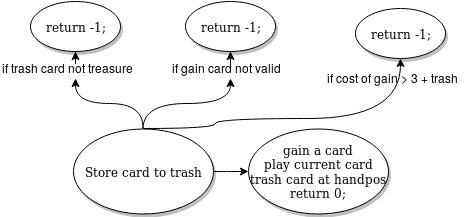
\includegraphics[width=\textwidth]{cardtest4}
        \item \textbf{Input Coverage and Boundary Cases}
          I tested three different inputs for my tests: 
          \begin{itemize}
            \item A case where a copper is trashed for a silver
            \item A case where a copper is trashed for a village (illegal)
            \item A case where an estate is trashed for a silver (illegal)
          \end{itemize}
          As mentioned above, a more thorough unit test would also check whether the function
            returns -1 for attempting to convert a copper into a gold. Moreover, 
            my tests do not check whether it permits silver or gold to be trashed, and since
            there are only three treasures, there is nothing stopping a unit test from 
            exhaustively covering these options. Moreover, I would like to test the following
            cases:
          \begin{itemize}
            \item A case where there are multiple Mine cards in hand. Does this create
              undesirable behavior?
            \item A case where there is only Mine card in hand.
            \item A case where the function is called when the hand is at MAX\_HAND number of cards (and therefore, hand would exceed MAX\_HAND)
          \end{itemize}
        \end{enumerate}

    \end{itemize}

\end{enumerate}
\end{document}
